% Template for PLoS
% Version 1.0 January 2009
%
% To compile to pdf, run:
% latex plos.template
% bibtex plos.template
% latex plos.template
% latex plos.template
% dvipdf plos.template

\documentclass[10pt]{article}

% amsmath package, useful for mathematical formulas
\usepackage{amsmath}
% amssymb package, useful for mathematical symbols
\usepackage{amssymb}

% graphicx package, useful for including eps and pdf graphics
% include graphics with the command \includegraphics
\usepackage{graphicx}

% cite package, to clean up citations in the main text. Do not remove.
\usepackage{cite}

\usepackage{color} 

% Use doublespacing - comment out for single spacing
%\usepackage{setspace} 
%\doublespacing


% Text layout
\topmargin 0.0cm
\oddsidemargin 0.5cm
\evensidemargin 0.5cm
\textwidth 16cm 
\textheight 21cm

% Bold the 'Figure #' in the caption and separate it with a period
% Captions will be left justified
\usepackage[labelfont=bf,labelsep=period,justification=raggedright]{caption}

% Use the PLoS provided bibtex style
\bibliographystyle{plos2009}

% Remove brackets from numbering in List of References
\makeatletter
\renewcommand{\@biblabel}[1]{\quad#1.}
\makeatother


% Leave date blank
\date{}

\pagestyle{myheadings}
%% ** EDIT HERE **


%% ** EDIT HERE **
%% PLEASE INCLUDE ALL MACROS BELOW

%% END MACROS SECTION

\begin{document}

% Title must be 150 characters or less
\begin{flushleft}
{\Large
\textbf{Transcriptome variation in response to Marek's disease virus early infection}
}
% Insert Author names, affiliations and corresponding author email.
\\
Likit Preeyanon$^{1}$
C. Titus Brown$^{1,2}$
Hans H. Cheng$^{3,\ast}$
\\
\bf{1} Microbiology and Molecular Genetics, Michigan State University, East Lansing, MI, USA
\\
\bf{2} Computer Science and Engineering, Michigan State University, East Lansing, MI, USA
\\
\bf{3} USDA, ARS, Avian Disease and Oncology Laboratory, East Lansing, MI, USA
\\
$\ast$ E-mail: Corresponding hans.cheng@ars.usda.gov
\end{flushleft}

% Please keep the abstract between 250 and 300 words
\section*{Abstract}
Marek's disease (MD) is caused by highly oncogenic Marek's disease virus (MDV).
Different MHC alleles have been associated with susceptibility and resistance to the disease.
However, chickens line 6 and 7 show significant phenotypic differences when chanllenged with
MDV even with the same MHC allele. Therefore, the major unanswered question is what genetic factors
underlie the susceptibility and resistance of line 6 and 7.
In this study, we identified differentially expressed genes and isoforms in response to Marek's disease infection
from chickens line 6 and 7 and performed pathway and functional analysis.
Results show that changes in expression of genes and isoforms involved in innate immune responses in line 6 may contribute
to resistance of the disease. We also identified many single nucleotide polymorphisms (SNPs) between
line 6 and 7 that may cause aberrant alternative splicing, which results in isoform with distictive functions.

% Please keep the Author Summary between 150 and 200 words
% Use first person. PLoS ONE authors please skip this step. 
% Author Summary not valid for PLoS ONE submissions.   
\section*{Author Summary}

\section*{Introduction}

Marek's disease is an economically significant chicken disease that affects a poultry industry worldwide.
Total of \$2 billion loss has been reported from outbreaks~\cite{}.
The disease is caused by highly oncogenic Marek's disease virus (MDV) which causes T-cell lymphoma.
Vaccination is effective in reducing incidence of tumor formation; however, current MD vaccines do not
prevent infection or horizontal spread of the virus.
Improper use of vaccines is a key factor that drives evolution of highly virulent strains in vaccinated
flocks.

Many studies have reported strong associations between MHC alleles and resistance and susceptibility of
the disease. For example, chickens with MHC allele B$^{21}$ is highly resistant in contrast to chickens with
B$^{16}$ allele.
However, chickens line 6 and 7 , even with common allele (B$^6$), exhibit different phenotypic response to
MD.
The major unanswered question is what genetic factors contribute to susceptibility and resistance of
the disease.

Although gene expression has been shown to have a high correlation with phenotypes in many studies~\cite{}.
Studies have shown that alternative splice forms play a significant role in many biological events and
isoform expression levels can provide better signatures for some diseases~\cite{zhang2013isoform}.
Regulation of alternative splicing by enhancers (ESE) and silencers (ESS) and their corresponding
binding motifs have been identified in some organisms including human.
Mutations that disrupt or create exonic splicing enhancers could alter splicing patterns leading to aberrant alternative splicing.
In fact, 15\% of mutations that cause genetic diseases affect pre-mRNA splicing.
A number of disease-associated single-nucleotide polymorphims in coding regions (cSNPs) that affect exon splicing enhancers (ESEs) and
silencers (ESSs) have been characterized~\cite{blencowe2000exonic, wang2007splicing}.
We hypothesized that SNPs between line 6 and 7, which are located in exons, are responsible for differential
expression of some isoforms between chicken line 6 and line 7.
We reported some genes that could be regulated by \textit{cis-}regulatory elements that may also play a role in
immune reponses.


% Results and Discussion can be combined.
\section*{Results and discussion}

\subsection*{Differential gene expression in response to MDV infection}

To extensively study gene and isoform expression, we incorporated \textit{Ensembl} gene models
release 73 with \textit{de novo} and a reference-guided transcriptome assembly to build custom
gene models.
The models, therefore, include both \textit{Ensembl} annotated transcripts
and putative transcripts and genes.
The advantage of using custom gene models is it allows an investigation of unannotated genes and
isoforms, which is necessary for in-depth transcriptome study of an immune system.

Many genes were found to be differentially expressed (DE) between control and infected
chickens in line 6 and line 7.
While the number of unique downregulated genes in both lines are approximately equal,
the number of unique upregulated genes in line 7 is much greater than in line 6 as shown
in figure~\ref{degenes_venn}.
Interestingly, some genes that were differentially expressed in both lines were
regulated in the opposite direction (table~\ref{tab:opposite}).
Among genes downregulated in line 6 but upregulated in line 7,
\textit{LL} (lung lectin) and \textit{SFTPA1}, which encode lectin proteins, are part of
lectin-complement pathway.
\textit{LIMS1} is involved in cell differentiation and proliferation and
\textit{PPARG} is a suppressor of \textit{NF$\kappa$B}-mediated proinflamatory response.
On the other hand, nearly all genes upregulated in line 6 but downregulated in line 7
are involved in cell survival such as mRNAs splicing, cell growth, and protein systhesis,
except CD7 whose function is involved in T cell-B cell interaction.
This difference suggests that even at this stage of infection in line 6, the lytic phase 
could be controlled or subsided because the viruses are driven to undergo latent infection early.
Therefore, genes important for recovery of cell damages are upregulated.
In comparison, the lytic phase in line 7 may still continue and as a result, genes involved in
immune responses are still upregulated.
In addition, type I interferon (\textit{IFN-$\gamma$} and \textit{IFN-$\beta$}) as well as \textit{INF-$\alpha$3} were found to be highly
upregulated in infected chickens in both line 6 and 7 (table~\ref{tab:cytokines}).
However, expressions of genes encoding their corresponding receptors
were not different in line 6, but upregulated in line 7.
This could also reflect the ongoing immune responses in line 7.

Some DE genes have been reported from previous Microarray studies were also found to be
differentially expressed in this study.
For example, B6.1 (Bu-1) gene is known to be down-regulated approximately 2.27 fold in susceptible
chicken with MHC allele B\textsuperscript{19} at 4 d.p.i~\cite{sarson2008transcriptional}.
It was also found to be down-regulated about 3-fold in line 7 (susceptible).
Similary, \textit{GMZA} gene reported to be upregulated across genetically different chickens
(B$^{19}$, B$^{21}$ alleles), was also found to be highly upregulated.
In contrast, some genes that have been reported to be highly expressed in resistant chickens were
downregulated in both lines. Those genes are \textit{AMIGO2, MMP13} and \textit{CLEC3B}, which were
found to be downregulated more than 2-fold~\cite{sarson2008transcriptional}.
% Several genes involved in innate immune response were differentially expressed in resistant chickens:
% \textit{DDT, NMU, VIPR2} and \textit{HSP5}. Of all those genes, only HSP5 was upregulated.
Other immune genes reported to be highly expressed in susceptible chickens (line 7$_{2}$) including
\textit{AVD, ART1, NOS2, CXCL13L2, MX1} and \textit{SOCS1}~\cite{smith2011systems}
were also found to be highly upregulated in both line 6 and 7.
However, our results show the similar expression pattern of \textit{IL6} and \textit{IL18}, which were
only upregulated in line 7 in early stage of infection (3-5 d.p.i).

In contrary, \textit{IL15} has been reported non differential-expressed between control and infected chickens in
line 6$_{1}$ and 7$_{2}$~\cite{kaiser2003differential}; however,
it was only upregulated in line 7 in our study.
Expression of \textit{IL15} is induced by \textit{TLR9}, which binds to non-methylated CpG
residues present in genomes of many DNA viruses, including herpes simplex virus.
This cytokine auto-regulates the expression of \textit{CD40}, which is
a transmembrane receptor required for activation of macrophages by CD4 T cells.
Consequently, \textit{CD40} was only upregulated in line 7 (data not shown).


\subsection*{Functional analysis of differntial-expressed genes}

To determine pathways that were perturbed during the infection, data were
analysed by GOSeq, which accounted for gene lengths bias unique for RNA-Seq data~\cite{young2010method}.
Significantly perturbed pathways (FDR $< 0.1$) from both lines that involved in
immune response include Toll-like receptor signaling pathway, cytokine-cytokine receptor interaction,
intestinal immune network for IgA production and cell adhesion molecules (CAMs).
Some other pathways important in response to viral infection and only significantly
enriched in line 7 include phagosome, apoptosis, RIG-I-like receptor signaling pathway,
NOD-like receptor signaling pathway and lysosome.
Figure~\ref{kegg_phagosome} is a pictorial example of differentially expressed genes in phagosome pathway.
Although MHC I gene (\textit{BF1}) was differentially expressed in both lines, other genes involved in
expressing newly synthesized MHC I were only upregulated in line 7
suggesting that new MHC I molecules were actively produced and expressed on cell surface.
Furthermore, gene ontology analysis of biological processes (GO:BP) shows that categories involved in
both adaptive and innate immune responses were enriched in line 7 (supplementary material).
On the other hand, only categories involved in innate immune responses were enriched in line 6.
In addition, enrichment of apoptosis pathway in line 7 indicates that the programmed
cell death could be induced by CTL response to eliminate the viruses.

At this stage of infection, our results suggest that lytic infection of MDV stimulates
both innate and the adaptive immune response, which leads to activation of T cells in line 7.
Only activated T cells are infected by MDV, therefore, the lytic phase could facilitate the spread of
the viruses by enhancing expansion of activated T cells.
In contrast, the immune response in line 6 could be able to drive the viruses to latency phase early
and only activate the adaptive immune response in a very short duration.
Due to cell-associate nature of MDV, the viruses transfer to T cells via cell-to-cell contact between B cells and
T cells during antigen presentation or B cells activation by T helper cells.
Therefore, it is beneficial for the host to restrain such contact.
However, it is not clear how chickens in line 6 control the lytic infection of MDV.
% Two mechanisms have been speculated to contribute to MD resistance.
% First innate immune responses could be highly effective and could activate
% strong adaptive immune responses that rapidly control viral replication and force the viruses to undergo latent phase.
% Second, innate immune resposnes itself could be highly effective in limiting viral replication~\cite{smith2011systems}.

\subsection*{Differential exon usage (DEU)}

Immune system is isoform-rich and many genes express different isoforms with distinctive functions in response to
stimuli such as stress, chemicals and infection.
Changes in expression of splice forms of immune related genes have been reported to be associated with increase
susceptibility and poor prognosis of diseases~\cite{lynch2004consequences}.
Studying differential isoform expression could therefore shed lights into inherent differences between 
line 6 and 7 that confer resistance or susceptibility to MD.

In the past decades, microarray technology has been used to study gene and isoform expressions in many studies, but
its sensitiviy for detection of structurally similar isoforms is low and known or predicted annotations
are required to design probes~\cite{kane2000assessment}.
Although RNA-Seq method can provide a reliable estimate of an exon expression compared to microarray~\cite{pan2008deep}
and is not constrained to those limitations, studying isoform
expressions using RNA-Seq is still not straightforward because of short read lengths.
Reads from current Illumina technology are generally not long enough to span across all exons in an isoform.
In most cases, only exons in close proximity are covered by the same read, which makes it
difficult to accurately predict a full structure of the isoform.
In addition, some genes are fused due to overlapping untranslated regions (UTRs),
which can also result in erroneous predicted isoform structures.

Due to those issues, it is not feasible to accurately estimate exression of isoforms, especially when
gene annotation is constructed from \textit{de novo} assembly~\cite{trapnell2013differential}.
To avoid these issues, we chose to study exon expression instead of isoform expression.
Using MISO with exon-centric method, only reads spanning across a few exons are used and only exons
involved in a splicing event are examined.
The expression of exon inclusion is calculated as percent spliced in (Psi or $\Psi$), which can be used to
infer the portion of transcripts that include the exon in each sample~\cite{Katz:2010iv}.
In this study, we investigated the three most common alternative splicing events in vertebrates, which are skipped
exons (SE), an alternative $3\prime$ (A3SS) and $5\prime$ (A5SS) splice site.

\subsubsection*{DEU genes in response to MDV}

List of DEU genes from line 6 that show difference in $\Psi$ greater than 0.20 when compared to line 7
in infected chickens is shown in table~\ref{tab:line67i_diff_line67u_one},~\ref{tab:line67i_diff_line67u_two}
and~\ref{tab:line67i_diff_line67u_three}.
Genes can be categorized roughly into four groups based on the pattern of $\Psi$ across control and
infected birds in both lines.

Group I includes genes that $\Psi$s were up or down regulated in infected chickens in line 6 only.
This group include \textit{BCL11B} (B-cell CLL/lymphoma 11B zinc finger proteins), a B-cell lymphoma
associated C2H2-type zinc finger protein encoding gene, which functions as a tumour-suppressor
in T-cell lymphoma in human.
According to homologous alignments on UCSC genome browser, a splice form with the skipped exon
is similar to mouse \textit{BCL11B isoform b}.
The skipped exon was expressed 30\% in infected line 6 chickens; whereas it was rarely expressed
(4-7\%) in the control line 6 and both groups in line 7.
The skipped exon was not found to encode any known protein domain, however, it is in the middle of
two adjacent C2H2-type finger protein domains.
Another gene related to B and T cell lymphoma is \textit{SIK2} (salt-inducible kinase 2).
This gene has been reported to have a negative effect on T cell lymphoma by limiting the transcription of
HTLV-1 virus~\cite{tang2013lkb1}.
Some other genes are important in pre-mRNA splicing including \textit{TRA2A}, \textit{SRSF6} and \textit{GEMIN6}.
\textit{TRA2A} (transformer-2 protein homolog alpha) encodes RNA recognition motif (RRM),
the skipped exon is not found to encode any known protein domain.
\textit{SRSF6} (SR splicing factor 6) encodes a nuclear protein that belongs to the splicing factor protein family.
\textit{GEMIN6} plays a role in the assembly of spliceosomal snRNP in cytoplasm.
These genes could play a significant role in regulating inclusion of alternative exons.
A gene in this group that might be important for innate immune responses is \textit{RAC3} (Ras-related C3
botulinum toxin substrate 3).
This gene encodes small GTPases, belonging to Ras family, that regulates a wide variety of cellular events
including cell growth, cytoskeletal reorganization and the activation of protein kinases.
The role of small GTPases in immune responses is discussed further below.

In group II, $\Psi$ values were relatively stable in control and infected chickens in line 6 and line 7.
Genes that could play an important role in immune responses are \textit{ITGB2} and \textit{HCK}.
\textit{ITGB2} (CD18) encodes subunit $\beta_{2}$ integrin of \textit{LFA-1} and \textit{CR3} receptors.
\textit{LFA-1} plays an important role in adhesion of lymphocytes with other cells.
\textit{CR3} binds to a vast array of ligands and molecules including complement C3bi, microbial proteins,
ICAM-1 and -2, ECM proteins and coagulation proteins~\cite{}.
It plays a significant role in neutrophils and monocytes activation including phagocytosis, adhesion and
migration~\cite{}.
Mutations in CD18 gene has been associated with type 1 leukocyte adhesion deficiency (LAD-1),
an autosomal-recessive inherited disease found in few families.
The disease is characterized by impair of lymphocytes in adherent-dependent functions, lack of accumulation
to the site of infection and recurrent bacterial and fungal infection~\cite{}.
\textit{HCK} transmits signal from cell surface receptors such as \textit{FCGR1A, FCGR2A, IL2, IL6,
IL18} and integrins (\textit{ITGB1, ITGB2}).
Based on our gene model, the skipped exon of \textit{ITGB2} is located in the 5$\prime$ UTR;
whereas, the skipped exon of \textit{HCK}, encodes protein tyrosine kinase (Pfam:PF07714).
Some other genes in this group are involved in cell rearrangement and cytokinesis that could be
regulated by signals from integrins including \textit{DYLNT1,DYNLL2, SEPT11, PFN2} and \textit{ZDHHC7}.
The role of \textit{ITGB2} in innate immune responses will be discuss further in the next section.

Group III includes genes that exhibit differential isoform expression only in infected chickens in line 7.
A number of genes in this group encode proteins that are parts of spliceosome: \textit{SRSF3}, \textit{HNRNPDL},
\textit{SFSWAP}, \textit{THOC1}, \textit{RNPC3} and \textit{SRSF5}.
Two genes involved in cell-cell contact regulated by integrins are also in this group.
\textit{PPP1R12A} is a myosin phosphatase that regulates the interaction of actin and myosin downstream of GTPase
Rho proteins.
\textit{PODXL} encodes protein that functions in integrin-dependent manner to increase cell-cell contact.
Connections of these two genes and integrins will be discussed in the next section.

The last group only has one gene, \textit{GOSR1}.
The $\Psi$ value of this gene was less than 0.20 cutoff in control and infected chickens in line 6, but it is
significantly different between infected chickens in line 6 and 7.
Also, there is a significant difference between control and infected chickens in line 7.
This gene encodes traffiking membrane protein important for transporting proteins from \textit{cis-} to
\textit{trans-}golgi network.

\subsubsection*{Integrins and actin cytoskeleton pathway}

Integrins are a special kind of receptors that transmit signals bidirectionally across cell membrane.
They are heterodimeric composed of an $\alpha$ (large) and a $\beta$ (small) subunits.
$\beta_{2}$ (CD18) subunit is exclusively expressed on lymphocytes and APCs as a component of \textit{LFA-1}
and \textit{CR3} receptors.

(more on \textit{LFA-1} and \textit{CR3} to be added).

As discussed above, \textit{RAC3, HCK, DYLNT1, DYNLL2, SEPT11, PFN2, ZDHHC7, PODXL} and \textit{PPP1R12A}
could be activated by the integrins because of their roles in cell rearrangement or molecular interaction.
Interestingly, we found that in human, \textit{RAC3, ITGB2, PFN2} and \textit{PPP1R12A} are in the regulation
of actin cytoskeleton pathway (figure~\ref{kegg_actin}).
Moreover, at least two of these genes are co-present in other three pathways (table~\ref{tab:integrin}) that
involved in immune responses.
This strongly suggests that these four genes could contribute to difference in immune responses between
line 6 and 7 even though their expressions were not significantly different between control and infected groups.

% \subsubsection*{Splicing factors}
% 
% (Not sure if I should write about splicing factors, I'm afraid it will make the paper too long and unfocused.)
% 
% The second group includes genes encode protein compoments of spliceosome or are involved in pre-mRNA splicing.
% Those genes are \textit{TRA2A, SRSF6, GEMIN6, SRSF3, HNRNPDL, SFSWAP, THOC1, THOC2, RNPC3} and \textit{SRSF5}.
% Even though alternative splicing is regulated by splicesome, it is difficult to elucidate the effect of alternative
% splice forms of spliceosome subunits on alternative splicing regulation.
% This is in part due to the fact that the spliceosome is the most complex protein structures composed of many different
% subunits each of which could have isoforms differing in function or activity~\cite{}.

\subsubsection*{Protein domains}
To understand the role of the alternative splice forms on the function of these genes, transcripts were
translated to protein sequences by ESTscan~\cite{}.
Protein sequences were then searched for annotated protein domains using InterProSearch~\cite{}.
Besides \textit{ITGB2}, other genes have alternative exons located in coding regions and could potentially affect
functional protein domains in some ways.
The exon with alternative 3$\prime$ splice site of \textit{RAC3} encode part of a protein domain identified as small GTPase of Ras subfamily
(ProSiteProfiles:PS5142 and SMART:SM00173).
Rac3 is highly homologous to Rac1 and has been reported to possess the ability of promoting membrane ruffling, transformation, activation of
c-Jun transcriptional activity and a co-activator of NF$\kappa$B~\cite{,werbajh2000rac}.
Activated Rac also regulates production of superoxide in neutrophils and macrophages.

The alternative exon of \textit{PFN2} seems to disrupt the coding sequence that encode profilin domain (Pfam:PF00235).
The profilin domain is essential for almost all orgamisms and its functions include regulating actin polymerization, controlling
complex network of molecular interaction and transmitting signals from small-GTPase pathway.
It also binds to Rac effector molecules and a number of other ligands~\cite{witke2004role}.
The skipped exon of \textit{PPP1R12A} encode part of a protein domain annotated as protein phosphatase 1 (PIRSF:PIRSF038141).

\subsubsection*{Prediction of \textit{cis}-regulatory elements in alternative splicing exons}

Although alternative splicing of genes in all groups could be regulated by \textit{cis-} and \textit{trans-}splicing factors,
genes in group II are more likely to be regulated by \textit{cis-}regulatory factors.
The ratios of isoform expression in this group were relatively stable within line, but were significantly different between lines.
Investigation of nucleotide differences within exons of line 6 and 7 could reveal a possible role of cSNPs in regulating
alternative splicing in this groups.
We obtained a sequence of an alternative exon from line 6 and used Human Splicing Finder (HSF) to determine whether SNPs from
line 7 could alter predicted ESEs or ESSs.
SNPs in exons of \textit{ITGB2} and \textit{PFN2} between line 6 and 7 are listed in table~\ref{tab:deu_snps}.

For \textit{ITGB2}, a putative ESE motif of SC35 is predicted to be broken when replace a T with a C at position 26 of the cDNA, which
corresponds to a position 7,183,696 on chromosome 7.
The disruption of this exon enhancer binding site support the fact that the level of exon inclusion in line 7 is
practically zero (figure~\ref{itgb2}).
On the other hand, there is also a putative binding site for an exon suppressor that could promote exclusion of the exon in line 7.
The SNP is also predicted to affect putative ESE motifs of other splicing factors, however, those motifs do not seem to agree with
exon expression data.

Exon sequences of \textit{PFN2} from line 6 and 7 differ at a position 2,072 on cDNA or 23,221,934 on chromsome 9.
A small insertion of two AA nucleotides is predicted to create a new ESE motif for Tra2-$\beta$ splicing regulator,
whose function as a stabilizer of an enhancer complex~\cite{lopez1998alternative}.
From exon expreesion data from, $\Psi$ of an exon with alternative splicing increases from 0.20-0.30 to about 0.50 in line 7.
Possibly, Tra2 increases inclusion of the exon with alternative 3$\prime$ splice site via
ESE-dependent 3$\prime$ splice site activation (figure~ref{pfn2}).
Even though the linear distance between Tra2-$\beta$ binding site and the alternative 3$\prime$ splice site is
greater than 1kb, Tra2 could bind close to the 3$\prime$ splice site if the secondary structure of the mRNA moves the
ESE motif closer to the splice site.

\section*{Discussion}


% You may title this section "Methods" or "Models". 
% "Models" is not a valid title for PLoS ONE authors. However, PLoS ONE
% authors may use "Analysis" 
\section*{Materials and Methods}
\subsection{Gene Models Construction}

Due to lack of complete gene models for chickens, we employed two methods to
construct gene models from RNA-Seq reads.
First, short reads were quality trimmed with conditri/2.1~\cite{}
and assembled using Velvet/1.21~\cite{} and Oases/0.2.06~\cite{} to obtain long transcripts.
Assembly was done with hash lengths range from 21 to 31 for both local and global assembly
(described in Gimme paper).
Poly-A tails were trimmed and low complexity transcripts were removed by Seqclean~\cite{}.
All transcripts were then aligned to chicken reference genome (galGal4, with unplaced and random 
chromosomes removed) with BLAT~\cite{}.
Second, reads were aligned to reference genome using Tophat/2.0.5~\cite{} and \textit{Ensemble} gene
models release 73 was used to guide reference-based assembly by Cufflinks2~\cite{}.
Alignments from BLAT and models from Cufflinks were then combined to construct gene models by Gimme
(manuscript in preparation).

\subsection{Differential Gene Expression and Gene Ontology}

To identify DE genes, reads were mapped to transcripts by RSEM v.1.10.1~\cite{li2011rsem}, which is
also used to estimate genes expression and identify DE genes.
Data from single- and paired-end datasets from the same line were treated as biological replicates.
To identify enriched pathways and ontology terms, a list of DE genes was analysed by GOSeq v.1.10.0 based on
chicken KEGG annotations.
P-values were corrected by Benjamini-Hochberg multiple testing correction.
Genes, patways and GO terms with corrected P-value $<0.1$ were considered significant.
Pathview~\cite{luo2013pathview} was used to create a KEGG pathway diagram with colors representing relative level of gene expressions.

\subsection{Differential Splicing Event}
Gene models were converted to alternative splicing models using a Python script.
In order to increase sensitivity, read counts from single- and paired-end samples were combined and treated
as single-end reads for splicing event analysis with MISO/0.4.9~\cite{Katz:2010iv}.
Splicing events with Bayes factor $>10$ and $\Delta\Psi>0.20$ were considered significant.
Read coverages and $\Psi$ distributions were plotted using Sashimi plot~\cite{Katz:2013vx}.

\subsection{Variant Calling and \textit{In Silico} Splicing Analysis}
Variants were called using mpileup command from SAMTools/0.1.18~\cite{} and BCFTools~\cite{}.
Only variants with quality score $\ge20$ were used for mutation analyses.
Exon enhancers and suppressors were predicted using Human Splicing Finder web portal~\cite{}.
Human default parameter settings were used in all analyses.
The following regulatory sequences were used to determined the effect of variants:
HSF integrated matrices for serine/arginine-rich proteins (SRp40, SC35, SF2/ASF, SF2/ASF,
IgM/BRCA1, and SRp55), exonic splicing enhancer (ESE), RESCUE-ESE hexamer (RESCUE-ESE),
putative 8-mer ESEs (PESEs) and putative 8-mers exonic splicing silencers (PESSs),
exon-identity and intron-identiry elements (EIEs and IIEs), hetronuclear ribonucleoprotein-binding
motifs, and Fas exonic splicing silencers.

\subsection{Protein domains search}

% Do NOT remove this, even if you are not including acknowledgments
\section*{Acknowledgments}

% \section*{References}
% The bibtex filename
\bibliography{ref}{}

\section*{Figure Legends}

\begin{figure}[!ht]
    \begin{center}
        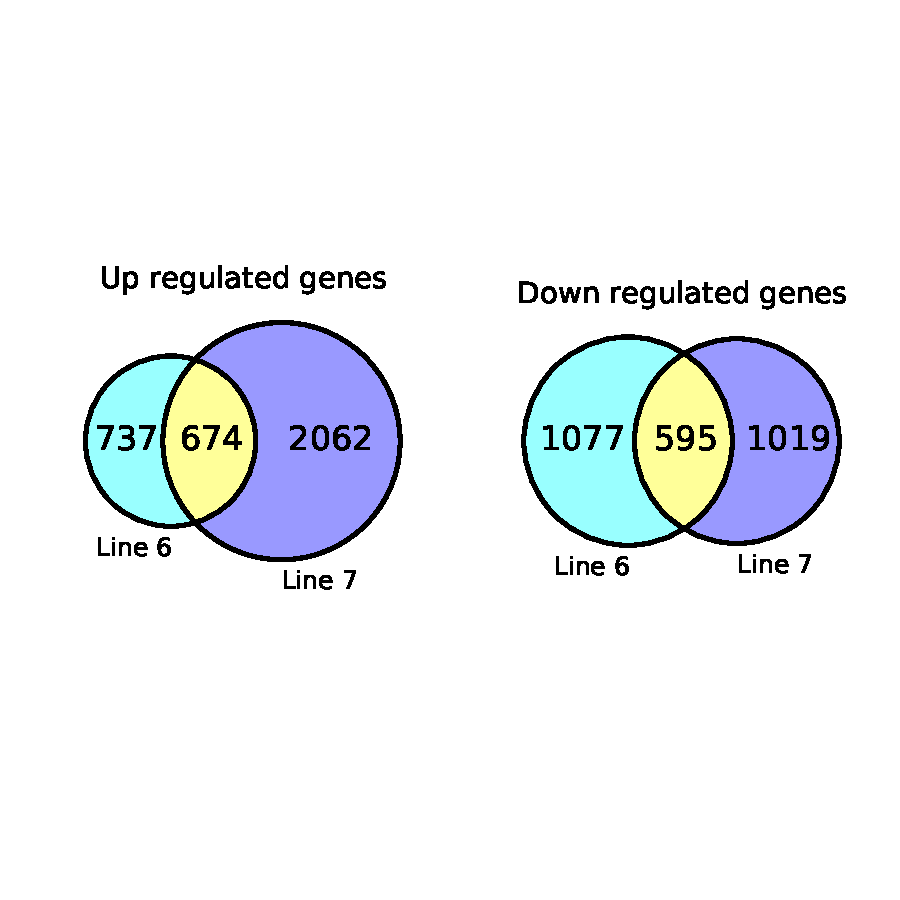
\includegraphics[width=6in]{degenes_venn.pdf}
    \end{center}
    \caption{
        {\bf Differential-expressed genes in response to MDV infection}
    }
    \label{degenes_venn}
\end{figure}

\begin{figure}[!ht]
    \begin{center}
        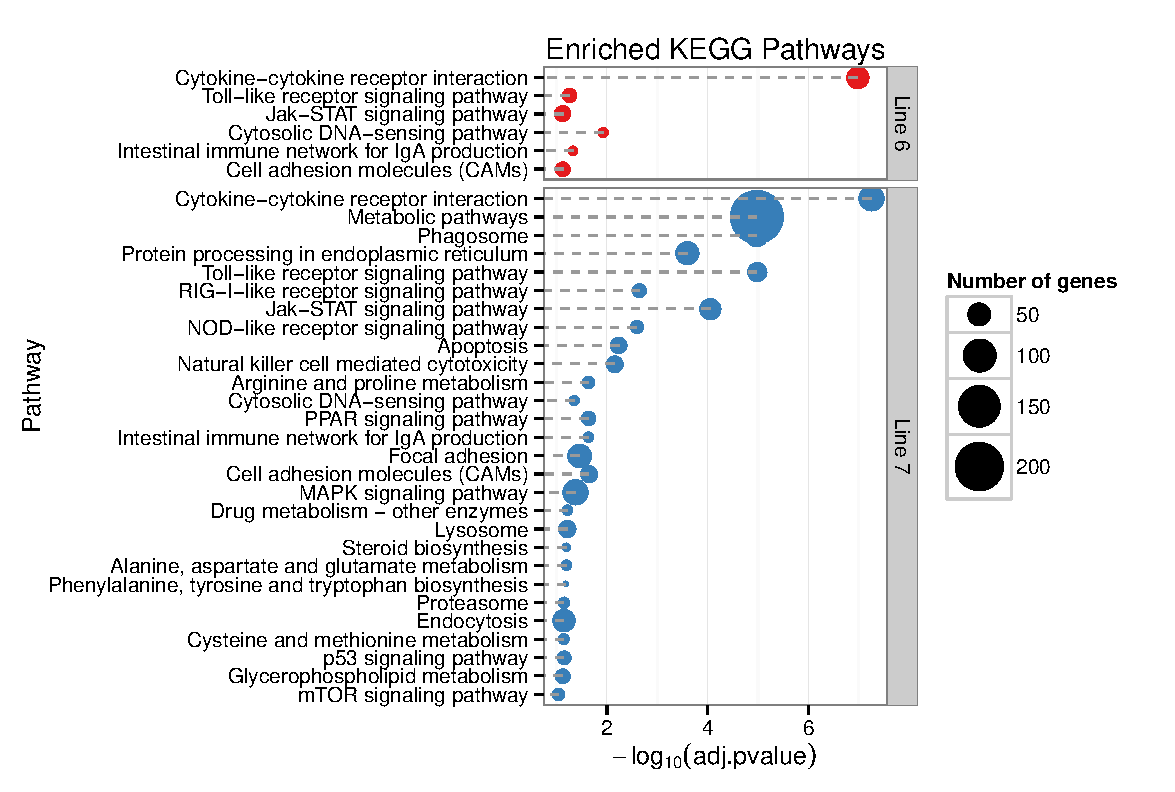
\includegraphics[width=7in]{line67_KEGG_cleveland.pdf}
    \end{center}
    \caption{
        {\bf Enriched KEGG pathways.}
    }
    \label{line67_kegg}
\end{figure}

\begin{figure}[!ht]
    \begin{center}
        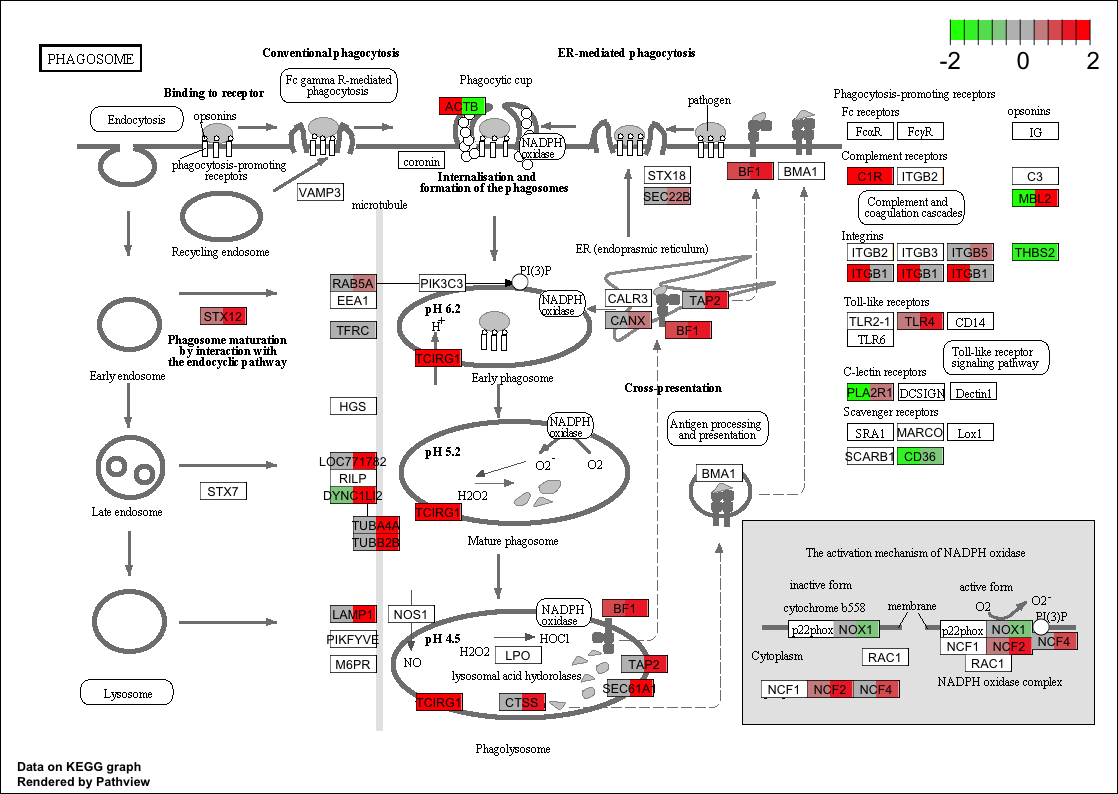
\includegraphics[width=6in]{gga04145_degenes_multi.png}
    \end{center}
    \caption{
        {\bf Phagosome pathway.}
    }
    \label{kegg_phagosome}
\end{figure}

\begin{figure}[!ht]
    \begin{center}
        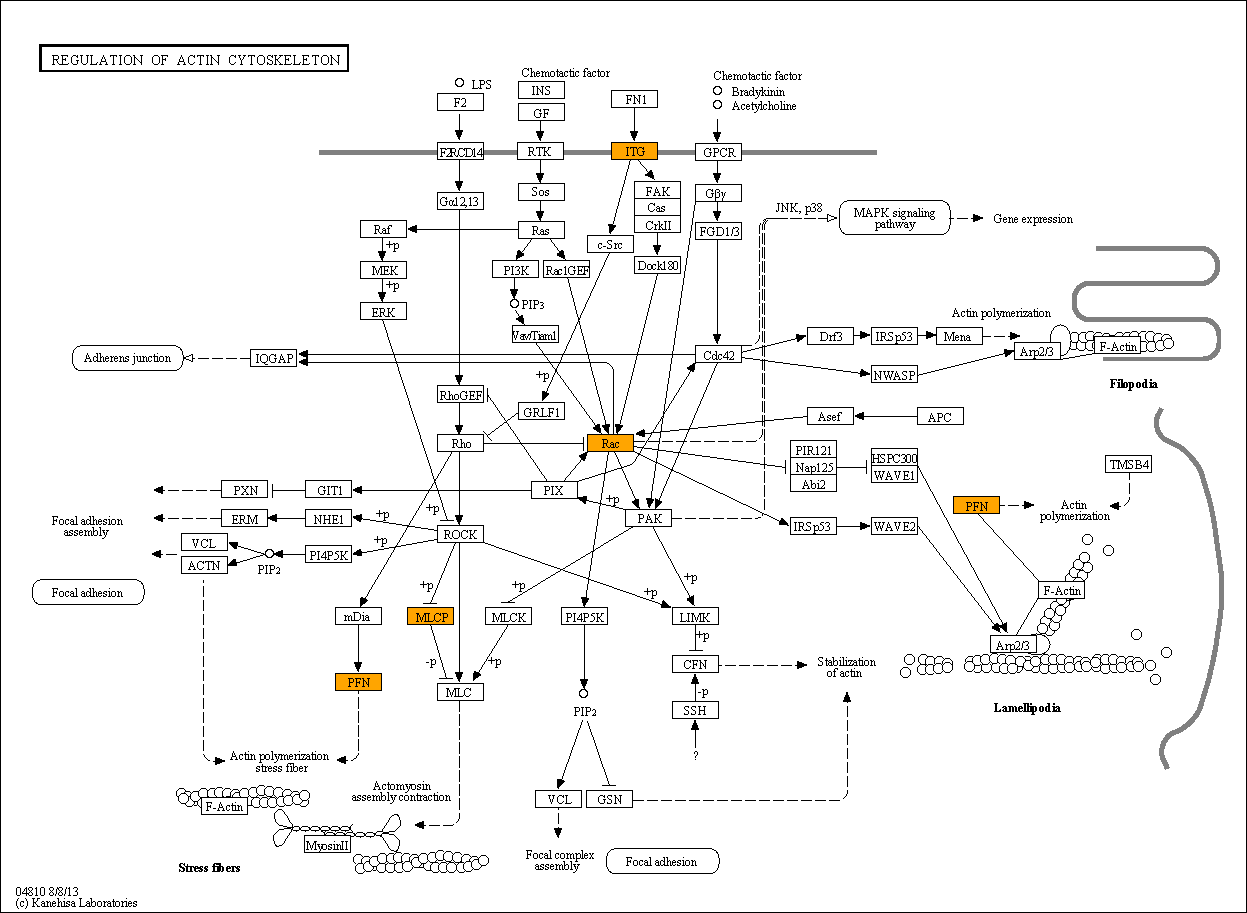
\includegraphics[width=6in]{hsa04810_deu_genes.png}
    \end{center}
    \caption{
        {\bf Human regulation of actin cytosekeleton pathway.}
    }
    \label{kegg_actin}
\end{figure}

\begin{figure}[!ht]
    \begin{center}
        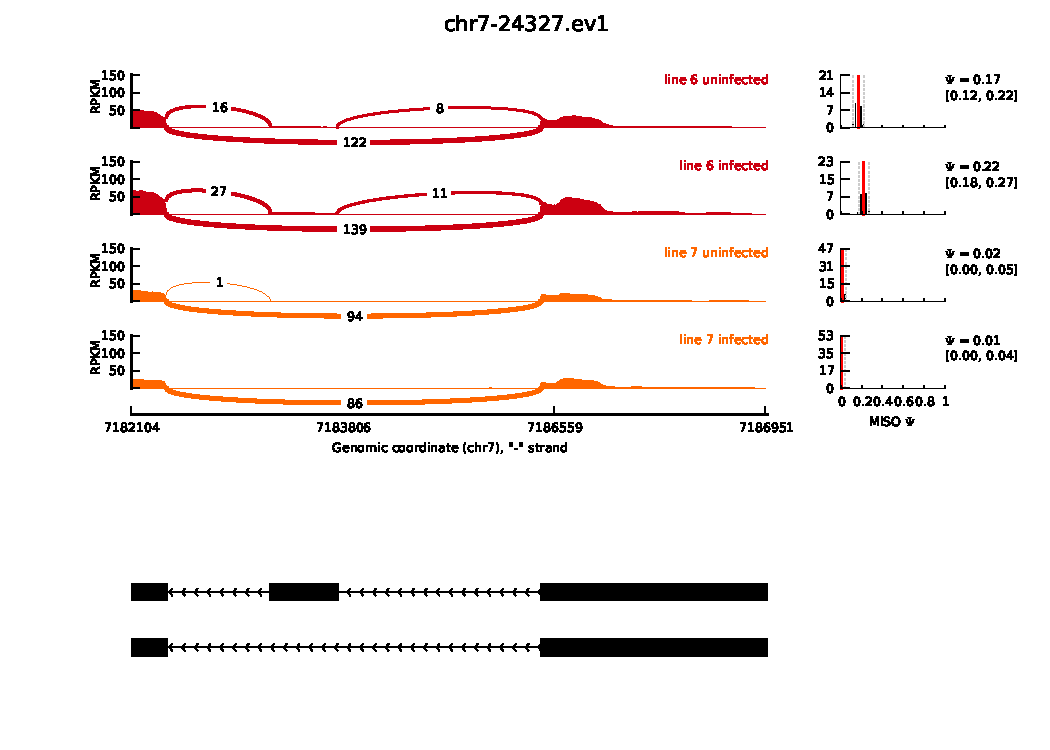
\includegraphics[width=6in]{itgb2_miso.pdf}
    \end{center}
    \caption{
        {\bf ITGB2 exon expression.}
        A single nuclotide substition (T$>$C) at position 7,183,696 is predicted to disrupt a putative ESE
        motif which binds SC35 on the skipped exon of IRGB2 gene shown in this figure.
        The prediction correlate with exclusion of the exon in line 7 ($\Psi \leq 0.02$).
        A new binding site for a silencer is also predicted and could also promote the exclusion of the exon. 
    }
    \label{itgb2}
\end{figure}

\begin{figure}[!ht]
    \begin{center}
        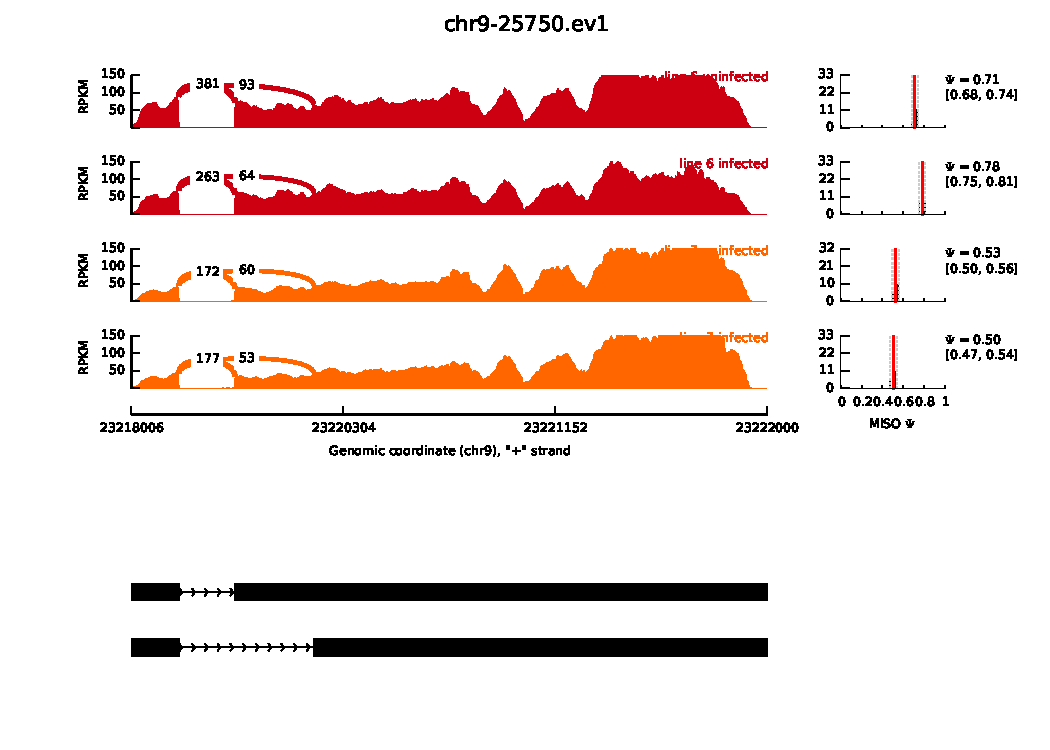
\includegraphics[width=6in]{pfn2_miso.pdf}
    \end{center}
    \caption{
        {\bf PFN2 exon expression.}
        A small insertion of AA nucleotides at position 23,221,934 is predicted to create a putative ESE motif
        which binds to Tra2 protein.
        Tra2 could promote inclusion of exon with alternative 3$\prime$ splice site via ESE-dependent
        3$\prime$ splice site activation resulting in higher expression of the exon in line 7.
        Even though the predicted ESE motif is located at a substantial distance from the alternative 3$\prime$ splice site,
        Tra2 could still regulate the splicing if a secondary structure of the mRNA moves the ESE motif closer to the
        alternative 3$\prime$ splice site.
    }
    \label{pfn2}
\end{figure}

\section*{Tables}

% \begin{table}[!ht]
%     \caption{
%     \bf{Gene models summary}}
%     \begin{tabular}{ccc}
%         \hline
%         Method & Gene & Isoform \\
%         \hline
%         Assembly & 25,290 & 54,044 \\
%         Cufflinks & 21,345 & 36,218 \\
%         Combined & 24,980 & 46,613 \\
%         \hline
%     \end{tabular}
%     \begin{flushleft}
%         Number of genes and isoforms from gene models
%         built from \textit{de novo} assembly and Cufflinks.
%         Combination of both methods decreased the number of genes
%         and isoforms by merging fragmented transcripts to
%         form more complete gene models.
%     \end{flushleft}
%     \label{tab:gene_models}
% \end{table}

\begin{table}[!ht]
\caption{
\bf{Genes regulated in opposite directions}}
    \begin{tabular}{cccc}
        \hline
        Gene & Description & $log_{2}$FC & \\
         & & Line 6 & Line 7 \\
        \hline
        LL & Lung lectin & -3.36 & 8.70 \\
        GIF & Gastric intrinsic factor & -2.15 & 3.11 \\
        SFTPA1 & Surfactant protein A1 & -4.84 & 3.73 \\
        SCAF8 & SR-related CTD-associated factor 8 & -8.70 & 8.24 \\
        LIMS1 & LIM and senescent cell antigen-like domains 1 & -2.26 & 1.33 \\
        PPARG & Peroxisome proliferator-activated receptor gamma & -6.99 & 2.06 \\
        C14ORF1 & Chromosome 14 open reading frame 1 & -3.11 & 2.71 \\
        Unknown & Unknown & -3.08 & 1.62 \\
        \hline
        ATP8A2 & ATPase, aminophospholipid transporter, class I, type 8A, member 2 & 7.66 & -7.80 \\
        S1PR1 & Sphingosine-1-phosphate receptor 1 & 1.31 & -6.95 \\
        MED9 & Mediator complex subunit 9 & 8.22 & -3.15 \\
        DNAJA2 & DnaJ (Hsp40) homolog, subfamily A, member 1 & 2.34 & -6.02 \\
        RAD17 & RAD17 homolog (S. pombe) & 1.45 & -1.80 \\
        PSMG3 & Proteosome assembly chaperone 3 & 1.52 & -1.26 \\
        PNISR & PNN-interacting serine/argining-rich protein & 5.58 & -1.81 \\
        THOC7 & THO complex 7 homolog (Drosophila) & 7.00 & -6.90 \\
        YTHDC2 & YTH domain containing 2 & 1.00 & -1.74 \\
        RPL39 & Ribosomal protein L39 & 3.31 & -1.59 \\
        CD7 & CD7 molecule & 2.88 & -1.38 \\
        NDUFB3 & NADH dehydrogenase (uqiquinone) 1 beta subcomplex 3 & 1.03 & -1.34 \\
        LOC100858785 & Unknown & 1.26 & -1.75 \\
        Unknown & Unknown & 6.30 & -5.22 \\
        \hline
    \end{tabular}
    \begin{flushleft}
        (-) down-regulated, (+) up-regulated
    \end{flushleft}
    \label{tab:opposite}
\end{table}

\begin{table}[!ht]
\caption{
\bf{Cytokine-related gene expression in response to MDV infection}}
    \begin{tabular}{cccccc}
        \hline
        & & $log_{2}$FC & \\
        Symbol & Description & Line 6 & Line 7 \\
        \hline
        IL2RG & Interleukin 2 receptor, $\gamma$ & -- & 0.55 \\
        IL6 & Interleukin 6 (interferon, $\beta$ 2) & -- & 5.15 \\
        IL6ST & Interleukin 6 signal transducer (gp130, oncostatin M receptor) & -- & 1.36 \\
        IL8L1 & Interleukin 8-like 1 & 1.90 & -- \\
        IL15 & Interleukin 15 & -- & 1.06 \\
        IL18 & Interleukin 18 (interferon-$\gamma$ inducing factor) & 1.92 & 4.06 \\
        IL18R1 & Interleukin 18 receptor 1 & 1.94 & 1.64 \\
        IFNG & Interferon-$\gamma$ & 5.14 & 4.90 \\
        IFNB & Interferon-$\beta$ & 4.83 & 5.64 \\
        IFNA3 & Interferon-$\alpha$ 3 & 4.09 & 5.48 \\
        IFNGR1 & Interferon-$\gamma$ receptor 1 & -- & 2.05 \\
        IFNGR2 & Interferon-$\gamma$ receptor 2& -- & 0.50 \\
        IFNAR1 & Interferon-$\alpha$,$\beta$ receptor 1 & -- & 1.46 \\
        IFNAR2 & Interferon-$\alpha$,$\beta$ receptor 2 & -- & 0.58 \\
        \hline
    \end{tabular}
    \begin{flushleft}
    \end{flushleft}
    \label{tab:cytokines}
\end{table}

\begin{table}[!ht]
\caption{
\bf{DEU between Line 6 and Line 7 in infected birds group I}}
\begin{tabular}{cccccccc}
\hline
& & & & Line 6 ($\Psi$) & & Line 7 ($\Psi$) & \\
Type & Event ID & Ensembl & Symbol  & Un & Inf & Un & Inf \\
\hline
SE & chr2:13729.ev2 & ENSGALG00000010973 & \textbf{TRA2A} & 0.45 & \textbf{0.75} & 0.58 & 0.50 \\
SE & chr5:22858.ev1 & ENSGALG00000011127 & BCL11B & 0.07 & \textbf{0.30} & 0.06 & 0.04 \\
SE & chr2:13065.ev1 & ENSGALG00000013137 & INO80C & 0.14 & \textbf{0.35} & 0.96 & 0.86 \\
SE & chr20:14995.ev1 & ENSG00000124193* & SRSF6 & 0.43 & \textbf{0.72} & 0.54 & 0.34 \\
A5SS & chr7:24049.ev1 & ENSGALG00000009824 & \textbf{C7H2ORF77} & 0.50 & \textbf{0.73} & 0.32 & 0.38 \\
A5SS & chr3:18098.ev1 & ENSGALG00000013821 & \textbf{GEMIN6} & 0.84 & \textbf{0.61} & 0.81 & 0.85 \\
A3SS & chr1:6450.ev1 & ENSGALG00000027665 & \textbf{SYNGR1} & 0.46 & \textbf{0.22} & 0.68 & 0.60 \\
A3SS & chr2:13270.ev1 & ENSGALG00000026498 & \textbf{Unknown} & 0.12 & \textbf{0.71} & 0.10 & 0.34 \\
A3SS & chr19:12399.ev1 & ENSGALG00000005685 & \textbf{KSR1} & 0.23 & \textbf{0.56} & 0.28 & 0.35 \\
A3SS & chr1:6437.ev1 & ENSGALG00000012050 & \textbf{TNRC6B} & 0.57 & \textbf{0.39} & 0.95 & 0.93 \\
A3SS & chr18:11800.ev1 & ENSGALG00000002859 & \textbf{RAC3} & 0.31 & \textbf{0.15} & 0.33 & 0.39 \\
\hline
\end{tabular}
\begin{flushleft}
    *human homologs, Un=uninfected, Inf=infected.
    Bold face indicates that there is a SNP between line 6 and 7 within an alternative exon.
\end{flushleft}
\label{tab:line67i_diff_line67u_one}
\end{table}

\begin{table}[!ht]
\caption{
\bf{DEU between Line 6 and Line 7 in infected birds group II}}
\begin{tabular}{cccccccc}
\hline
& & & & Line 6 ($\Psi$) & & Line 7 ($\Psi$) & \\
Type & Event ID & Ensembl & Symbol  & Un & Inf & Un & Inf \\
\hline
SE & chr17:11370.ev2 & ENSGALG00000004971 & URM1 & \textbf{0.07} & \textbf{0.03} & 0.18 & 0.23 \\
SE & chr2:12495.ev3 & ENSGALG00000005582 & \textbf{KLHL18} & \textbf{0.44} & \textbf{0.27} & 0.56 & 0.52 \\
SE & chr7:24327.ev1 & ENSGALG00000007511 & \textbf{ITGB2} & \textbf{0.17} & \textbf{0.22} & 0.02 & 0.01 \\
SE & chr2:12984.ev1 & ENSGALG00000012809 & ECI2 & \textbf{0.15} & \textbf{0.29} & 0.58 & 0.49 \\
SE & chr8:25247.ev1 & ENSGALG00000028790 & DNASE2B & \textbf{0.38} & \textbf{0.50} & 0.29 & 0.26 \\
SE & chr1:4653.ev1 & ENSGALG00000011682 & CNOT4 & \textbf{0.57} & \textbf{0.63} & 0.40 & 0.40 \\
SE & chr20:14907.ev3 & ENSGALG00000006522 & \textbf{HCK} & \textbf{0.46} & \textbf{0.59} & 0.99 & 0.97 \\
SE & chr4:21539.ev1 & ENSGALG00000015709 & \textbf{TACC3} & \textbf{0.87} & \textbf{0.94} & 0.76 & 0.72 \\
SE & chr2:32201.ev1 & ENSGALG00000012258 & GOLGA4 & \textbf{0.33} & \textbf{0.34} & 0.51 & 0.61 \\
SE & chr3:19470.ev1 & ENSGALG00000019979 & DYNLT1 & \textbf{0.23} & \textbf{0.22} & 0.02 & 0.02 \\
SE & chr19:12391.ev1 & ENSGALG00000005522 & \textbf{DYNLL2} & \textbf{0.01} & \textbf{0.02} & 0.19 & 0.25 \\
A5SS & chr6:23812.ev1 & ENSG00000107651* & \textbf{SEC23IP} & \textbf{0.02} & \textbf{0.12} & 0.50 & 0.43 \\
A5SS & chr2:12775.ev1 & ENSGALG00000011488 & \textbf{CMTM7} & \textbf{0.55} & \textbf{0.67} & 0.37 & 0.41 \\
A3SS & chr8:25257.ev1 & ENSGALG00000008939 & \textbf{FUBP1} & \textbf{0.58} & \textbf{0.74} & 0.41 & 0.46 \\
A3SS & chr9:25750.ev1 & ENSGALG00000010410 & \textbf{PFN2} & \textbf{0.71} & \textbf{0.78} & 0.53 & 0.50 \\
A3SS & chr4:21230.ev1 & ENSGALG00000011476 & \textbf{SEPT11} & \textbf{0.22} & \textbf{0.14} & 0.40 & 0.42 \\
A3SS & chr4:20185.ev1 & ENSGALG00000008507 & THOC2 & \textbf{0.48} & \textbf{0.47} & 0.31 & 0.22 \\
A3SS & chr11:8703.ev1 & ENSGALG00000020987 & \textbf{ZDHHC7} & \textbf{0.42} & \textbf{0.23} & 0.57 & 0.55 \\
A3SS & chr4:21136.ev1 & ENSGALG00000027908 & \textbf{LOC42228} & \textbf{0.72} & \textbf{0.61} & 0.87 & 0.91 \\
\hline
\end{tabular}
\begin{flushleft}
    *human homologs, Un=uninfected, Inf=infected.
    Bold face indicates that there is a SNP between line 6 and 7 within an alternative exon.
\end{flushleft}
\label{tab:line67i_diff_line67u_two}
\end{table}

\begin{table}[!ht]
\caption{
\bf{DEU between Line 6 and Line 7 in infected birds group III and IV}}
\begin{tabular}{cccccccc}
\hline
& & & & Line 6 ($\Psi$) & & Line 7 ($\Psi$) & \\
Type & Event ID & Ensembl & Symbol  & Un & Inf & Un & Inf \\
\hline
SE & chr12:8987.ev1 & ENSGALG00000008320 & EDEM1 & 0.96 & 0.99 & 0.91 & \textbf{0.72} \\
SE & chr4:20411.ev1 & ENSGALG00000023199 & HNRPDL & 0.39 & 0.40 & 0.30 & \textbf{0.18} \\
SE & chrZ:26257.ev1 & ENSGALG00000001745 & PSTPIP2 & 0.06 & 0.04 & 0.13 & \textbf{0.26} \\
SE & chr1:6316.ev3 & ENSG00000058272* & PPP1R12A & 0.99 & 0.97 & 0.96 & \textbf{0.77} \\
SE & chr1:4478.ev2 & ENSGALG00000009029 & TSPAN12 & 0.09 & 0.15 & 0.20 & \textbf{0.46} \\
SE & chr4:20075.ev1 & ENSGALG00000006157 & DDX26B & 0.67 & 0.61 & 0.58 & \textbf{0.84} \\
SE & chr6:23515.ev1 & ENSGALG00000003861 & HERC4 & 0.31 & 0.37 & 0.45 & \textbf{0.06} \\
SE & chr26:16840.ev1 & ENSGALG00000000533 & SRSF3 & 0.36 & 0.38 & 0.30 & \textbf{0.16} \\
SE & chr11:8507.ev2 & ENSGALG00000000904 & \textbf{C11H16ORF57} & 0.91 & 0.98 & 0.84 & \textbf{0.78} \\
SE & chr1:4323.ev1 & ENSGALG00000006409 & PODXL & 0.21 & 0.34 & 0.26 & \textbf{0.13} \\
SE & chrZ:26582.ev2 & ENSGALG00000014642 & LOC374195 & 0.60 & 0.57 & 0.70 & \textbf{0.81} \\
SE & chr6:23833.ev1 & ENSG00000175029* & CTBP2 & 0.38 & 0.38 & 0.23 & \textbf{0.12} \\
A5SS & chr15:10720.ev1 & ENSGALG00000002487 & \textbf{SFSWAP} & 0.58 & 0.73 & 0.55 & \textbf{0.41} \\
A5SS & chr7:24350.ev1 & ENSGALG00000008038 & \textbf{SF3B1} & 0.41 & 0.57 & 0.55 & \textbf{0.31} \\
A3SS & chr2:13147.ev1 & ENSGALG00000014915 & \textbf{THOC1} & 0.33 & 0.48 & 0.33 & \textbf{0.23} \\
A3SS & chr23:15908.ev1 & ENSGALG00000000720 & LOC419563 & 0.12 & 0.06 & 0.17 & \textbf{0.30} \\
A3SS & chr8:25157.ev1 & ENSGALG00000005162 & RNPC3 & 0.45 & 0.64 & 0.58 & \textbf{0.33} \\
A3SS & chrZ:27197.ev1 & ENSGALG00000000189 & \textbf{YTHDC2} & 0.44 & 0.59 & 0.42 & \textbf{0.32} \\
A3SS & chr23:15983.ev1 & ENSG00000163875* & \textbf{MEAF6} & 0.28 & 0.57 & 0.40 & \textbf{0.29} \\
A3SS & chr5:21970.ev1 & ENSGALG00000009421 & \textbf{SRSF5} & 0.55 & 0.72 & 0.54 & \textbf{0.39} \\
\hline
SE & chr27:17351.ev1 & ENSGALG00000001107 & GOSR2 & 0.73 & 0.92 & 0.38 & 0.60 \\
\hline
\end{tabular}
\begin{flushleft}
    *human homologs, Un=uninfected, Inf=infected.
    Bold face indicates that there is a SNP between line 6 and 7 within an alternative exon.
\end{flushleft}
\label{tab:line67i_diff_line67u_three}
\end{table}

% \begin{table}[!ht]
% \caption{
% \bf{DEU Genes in Spliceosome pathway}}
% \begin{tabular}{cccccc}
% \hline
% Gene ID &  Ensembl & Symbol  & $-log2$FC* & \\
%         & & & Line 6 & Line 7 \\
% \hline
% chr26:16840 & ENSGALG00000000533 & SRSF3 & 0.43 & 0.18 \\
% chr2:13147 & ENSGALG00000014915 & THOC1 & -- & 0.21 \\
% chr5:21970 & ENSGALG00000009421 & SRSF5 & -- & 0.18 \\
% chr2:13729 & ENSGALG00000010973 & TRA2A & -- & -- \\
% chr4:20185 & ENSGALG00000008507 & THOC2 & -- & -- \\
% chr7:24350 & ENSGALG00000008038 & SF3B1 & -- & -- \\
% \hline
% \end{tabular}
% \begin{flushleft}
%     * FDR $<$ 0.05
% \end{flushleft}
% \label{tab:spliceosome}
% \end{table}

\begin{table}[!ht]
\caption{
\bf{Pathways containing \textit{RAC3, ITGB2, PFN2} and \textit{PPP1R12A}}}
\begin{tabular}{ccc}
\hline
Pathway ID &  Description & Gene \\
\hline
hsa04810 & Regulation of actin cytoskeleton & \textit{RAC3, ITGB2, PPP1R12A, PFN2} \\
hsa04015 & RAP1 signaling pathway & \textit{RAC3, ITGB2, PFN2} \\
hsa04650 & Natural killer cells cytotoxicity & \textit{RAC3, ITGB2} \\
hsa05416 & Viral myocarditis & \textit{RAC3, ITGB2} \\
hsa04510 & Focal adhesion & \textit{RAC3, PPP1R12A} \\
\hline
\end{tabular}
\begin{flushleft}
\end{flushleft}
\label{tab:integrin}
\end{table}

\begin{table}[!ht]
\caption{
\bf{SNPs in exons}}
\begin{tabular}{ccccccc}
\hline
Gene &  Chromosome & Position & Reference & Line 6 & Line 7 & Strand \\
\hline
ITGB2 & 7 & 7183696 & C & \textit{T} & C & - \\
PFN2 & 9 & 23221934 & -  - & - - & \textit{AA} & + \\
\hline
\end{tabular}
\begin{flushleft}
\end{flushleft}
\label{tab:deu_snps}
\end{table}

\begin{table}[!ht]
\caption{
\bf{Results from human splicing finder}}
\begin{tabular}{|l|p{1cm}|p{3cm}|l|l|l|l|}
\hline
Gene &  cDNA Position & Linked SR protein & Type & Reference Motif & Mutant Motif & Variation \\
\hline
ITGB2 & 20 & SC35 & ESE$^{1}$ & TGCTCATG (78.19) & & Site broken \\
 & 22 & SF2/ASF(IgM-BRCA1) & ESE$^{1}$ & CTCATGG (77.23) & CTCACGG (91.15) & +18.03\% \\
 & 22 & SF2/ASF(IgM-BRCA1), SF2/ASF & ESE$^{1}$ & CTCATGG (77.23) & CTCACGG (89.23) & +15.53\% \\
 & 22 & SF2/ASF, SF2/ASF(IgM-BRCA1) & ESE$^{1}$ & CTCATGG (74.55) & CTCACGG (91.15) & +22.27\% \\
 & 22 & SF2/ASF, SF2/ASF & ESE$^{1}$ & CTCATGG (74.55) & CTCACGG (89.23) & +19.69\% \\
 & 24 & SRp55 & ESE$^{1}$ & & CACGGA (79.30) & New site \\
 & 26 & SF2/ASF(IgM-BRCA1) & ESE$^{1}$ & & CGGAGAT (80.00) & New site \\
 & 26 & SF2/ASF & ESE$^{1}$ & & CGGAGAT (75.36) & New site \\
 & 21 & & ESS$^{3}$ & & GCTCACGG (63.35) & New site (-5.59) \\
 & 23 & & ESS$^{3}$ & TCATGGAG (61.41) & & Site broken (3.16) \\
 & 23 & & ESS$^{3}$ & ATGGAGAT (64.83) & ACGGAGAT & -5.16\% \\
 & 24 & & ESS$^{4}$ & CATGGA (65.48) & CACGGA (65.48) & 0\% \\
\hline
PFN2 & 2068 & Tra2-$\beta$ & ESE$^{1}$ & AAAAT (81.02) & AAAAa & +16.19\% \\
& 2069 & Tra2-$\beta$ & ESE$^{1}$ & & AAAaa (94.14) & New site \\
& 2070 & Tra2-$\beta$ & ESE$^{1}$ & & AAAaaT (81.02) & New site \\
 & 2066 & & ESS$^{2}$ & & ACAAAAaa (38.13) & New site \\
 & 2067 & & ESS$^{2}$ & & CAAAAaaT (28.85) & New site \\
\hline

\end{tabular}
\begin{flushleft}
    $^{1}$ESE Finder matrices for SRp40, SC35, SF2/ASF and SRp55 proteins.
    $^{2}$Predicted PESS Octamers from Zhang \& Chasin.
    $^{3}$Silencer motif from Sironi et al.
    $^{4}$hnRNP motif.
\end{flushleft}
\label{tab:spliceosome}
\end{table}

\end{document}
